\section{Исследования}
\subsection{Тестовое множество}
\subsubsection{Изображения}
Для исследования были взяты изображения из открытой базы данных ImageNet, а так же из личной коллекции. Была произведенна следующая классификация:
\begin{itemize}
	\item Изображения людей
	\item Изображения архитектуры
	\item Изображения полученные при недостаточной освещенности
\end{itemize}
Данная классификация обусловлена распространенностью данных классов изображений и прикладных задачах в области обработки изображений. Фотографии людей используются как в повседневной жизни, так и во многих алгоритмах компьютерного зрения, таких как например распознавание лиц.

Не менее распространенны так же и изображения полученные при недостаточной освещенности, что приводит к низко контрастному изображению. Это мешает их анализу. Так же данные это актуально и для обычных пользователей фото и видеокамер, устройство которых все еще не позволяет достичь приемлимых результатов при съемке ночью. 

Последняя категория была выбрана в качестве примера, где  некоторые части изображения похожи друг на друга. Это может быть полезно в таких областях связанных с медициной, электроникой и астрономией. Где изображения, необходимы для последующей обработки имеют подобные свойства.

Ниже приведены примеры изображений из каждой категории.

\begin{figure}[H]
	\begin{minipage}[H]{0.49\linewidth}
		\center{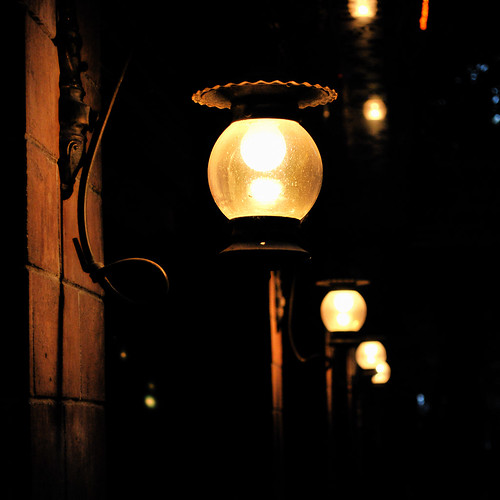
\includegraphics[scale=0.5]{imageNight} \\ а) Ночная съемка}
	\end{minipage}
	\begin{minipage}[H]{0.49\linewidth}
		\center{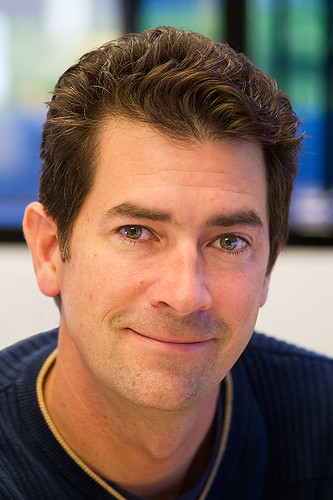
\includegraphics[scale=0.5]{imagePerson} \\ б) Человек}
	\end{minipage}
\begin{center}
	\begin{minipage}[H]{0.49\linewidth}
		\center{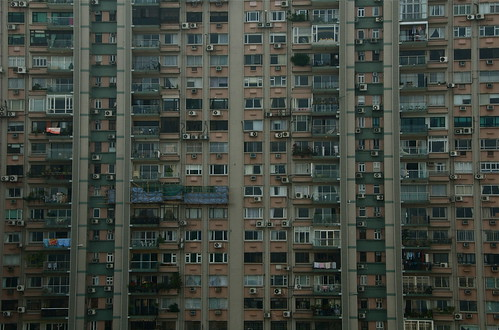
\includegraphics[scale=0.5]{imageArchitecture} \\ в) Архитектура}
	\end{minipage}
\end{center}
	\caption{Примеры изображений различных категорий}
\end{figure}


\subsubsection{Видео}
Данные необходимые для исследования видео последовательность были взяты из открытой базы данных  YouTube-8M\cite{youtube8m}.


Ниже приведены кадры из видео каждой категории.
\begin{figure}[H]
	\begin{minipage}[H]{0.49\linewidth}
		\center{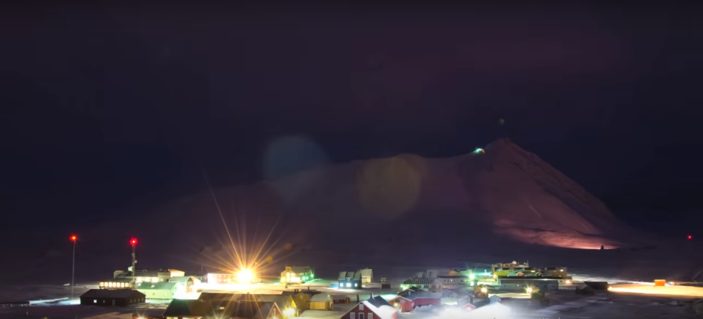
\includegraphics[trim={1.5cm 0cm 1.5cm 0cm},scale=1,clip]{videoNight} \\ а) Ночная съемка}
	\end{minipage}
	\begin{minipage}[H]{0.49\linewidth}
		\center{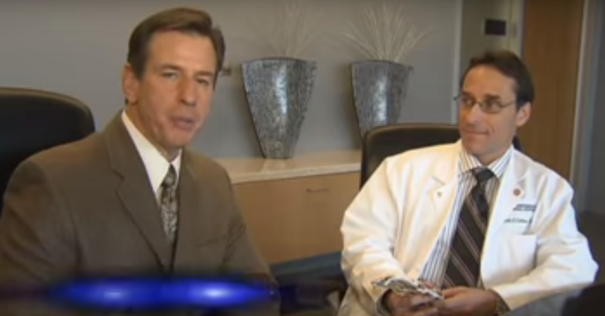
\includegraphics[trim={1.5cm 0cm 1.5cm 0cm},scale=1,clip]{videoPerson} \\ б) Человек}
	\end{minipage}
\begin{center}
		\begin{minipage}[H]{0.49\linewidth}
			\center{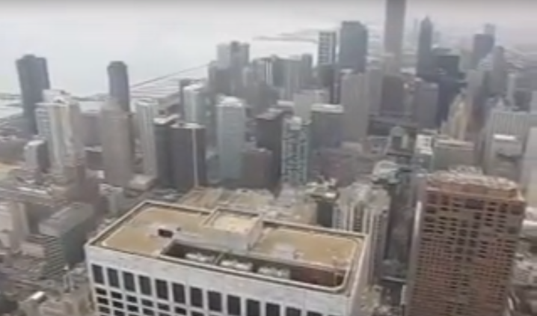
\includegraphics[]{videoArchitecture} \\ в) Архитектура}
		\end{minipage}
\end{center}
	\caption{Примеры кадров видео различных категорий}
\end{figure}
\subsection{Схема программы}
Работу реализованной программы можно описать следующим образом. На вход программы подаются данные (видео или изображение). Далее накладывается гауссовский шум. После проводится шумоподавления различными алгоритмами с различными параметрами. В итоге выбирается алгоритм, которые показал наибольшие показатели PSNR и SSIM. 
\begin{figure}[H]
	\center{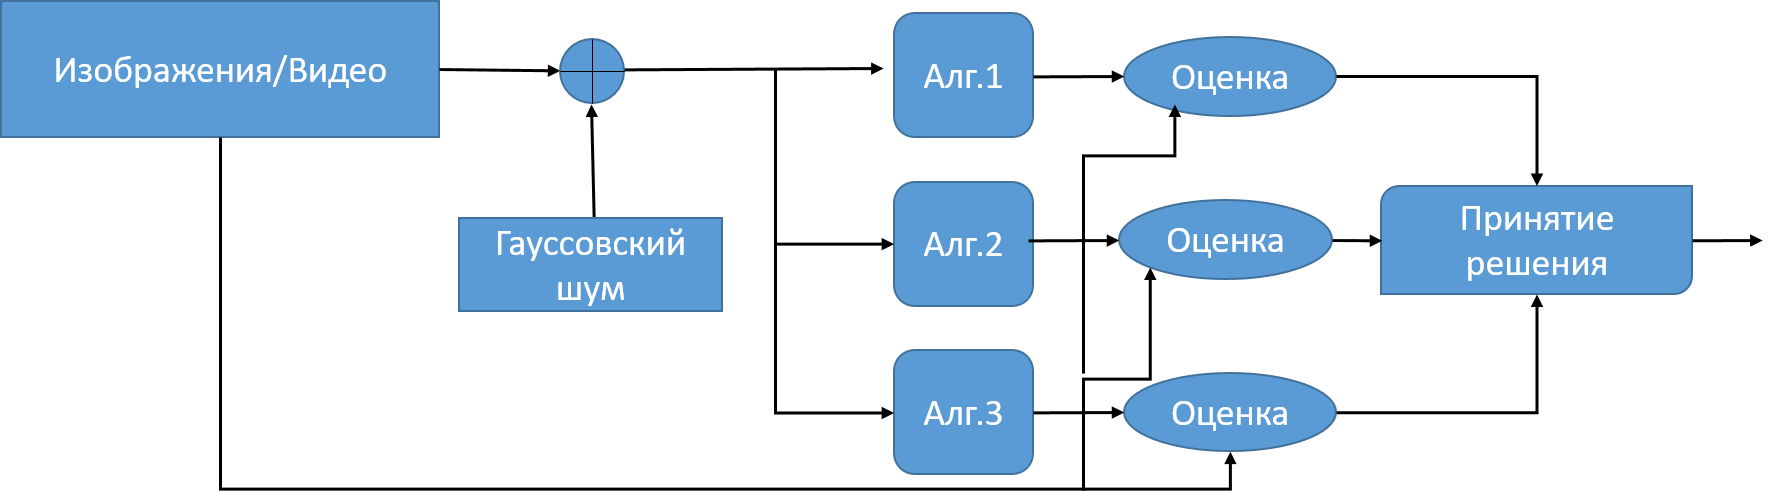
\includegraphics[scale=0.5]{circuitProgram}}
	\caption{Схема итоговой программы}
\end{figure}
\subsection{Результаты исследования}
Исследование разбито на две части. В первой части для каждого алгоритма подбираются оптимальные параметры, которые дают максимальной значение PSNR или SSIM для определенного типа изображения или видео. Исходя уже из полученных результатов будут сравниваться между собой все алгоритмы.
\subsubsection{Изображения}
Ниже представлены таблицы с результатами для каждой категории изображений, с различным количеством аддитивного гауссовского шума.
\begin{table}[H]
	\caption{\label{tab:bolts} Результаты для категории: человек.}
\begin{tabular}{|c|c|c|c|c|c|c|c|c|}
	\hline
	Название алгоритм & \multicolumn{2}{|c|}{$\sigma=0.005$}  & \multicolumn{2}{|c|}{$\sigma=0.01$}& \multicolumn{2}{|c|}{$\sigma=0.1$} & \multicolumn{2}{|c|}{$\sigma=0.4$} \\
	\cline{2-9}
	 & SSIM  & PSNR & SSIM  & PSNR & SSIM  & PSNR & SSIM  & PSNR\\
	\hline
	Bilateral & 0 & 0& 0 & 0& 0 & 0 & 0 & 0 \\
	\hline
	Guided & 0 & 0& 0 & 0& 0 & 0 & 0 & 0 \\
	\hline
	Non-local mean & 0 & 0& 0 & 0& 0 & 0 & 0 & 0 \\
	\hline
	TV & 0 & 0& 0 & 0& 0 & 0 & 0 & 0 \\
	\hline
	BM3D & 0 & 0& 0 & 0& 0 & 0 & 0 & 0 \\
	\hline	
\end{tabular}
\end{table}

\begin{table}[H]
	\caption{\label{tab:bolts} Результаты для категории: архитектура.}
	\begin{tabular}{|c|c|c|c|c|c|c|c|c|}
		\hline
		Название алгоритм & \multicolumn{2}{|c|}{$\sigma=0.005$}  & \multicolumn{2}{|c|}{$\sigma=0.01$}& \multicolumn{2}{|c|}{$\sigma=0.1$} & \multicolumn{2}{|c|}{$\sigma=0.4$} \\
		\cline{2-9}
		& SSIM  & PSNR & SSIM  & PSNR & SSIM  & PSNR & SSIM  & PSNR\\
		\hline
		Bilateral & 0 & 0& 0 & 0& 0 & 0 & 0 & 0 \\
		\hline
		Guided & 0 & 0& 0 & 0& 0 & 0 & 0 & 0 \\
		\hline
		Non-local mean & 0 & 0& 0 & 0& 0 & 0 & 0 & 0 \\
		\hline
		TV & 0 & 0& 0 & 0& 0 & 0 & 0 & 0 \\
		\hline
		BM3D & 0 & 0& 0 & 0& 0 & 0 & 0 & 0 \\
		\hline	
	\end{tabular}
\end{table}

\begin{table}[H]
	\caption{\label{tab:bolts} Результаты для категории: ночная съемка.}
	\begin{tabular}{|c|c|c|c|c|c|c|c|c|}
		\hline
		Название алгоритм & \multicolumn{2}{|c|}{$\sigma=0.005$}  & \multicolumn{2}{|c|}{$\sigma=0.01$}& \multicolumn{2}{|c|}{$\sigma=0.1$} & \multicolumn{2}{|c|}{$\sigma=0.4$} \\
		\cline{2-9}
		& SSIM  & PSNR & SSIM  & PSNR & SSIM  & PSNR & SSIM  & PSNR\\
		\hline
		Bilateral & 0 & 0& 0 & 0& 0 & 0 & 0 & 0 \\
		\hline
		Guided & 0 & 0& 0 & 0& 0 & 0 & 0 & 0 \\
		\hline
		Non-local mean & 0 & 0& 0 & 0& 0 & 0 & 0 & 0 \\
		\hline
		TV & 0 & 0& 0 & 0& 0 & 0 & 0 & 0 \\
		\hline
		BM3D & 0 & 0& 0 & 0& 0 & 0 & 0 & 0 \\
		\hline	
	\end{tabular}
\end{table}

\subsubsection{Видео}
Ниже представлены таблицы с результатами для каждой категории видео, с различным количеством аддитивного гауссовского шума.
\begin{table}[H]
	\caption{\label{tab:bolts} Результаты для категории: человек.}
	\begin{tabular}{|c|c|c|c|c|c|c|c|c|}
		\hline
		Название алгоритм & \multicolumn{2}{|c|}{$\sigma=0.005$}  & \multicolumn{2}{|c|}{$\sigma=0.01$}& \multicolumn{2}{|c|}{$\sigma=0.1$} & \multicolumn{2}{|c|}{$\sigma=0.4$} \\
		\cline{2-9}
		& SSIM  & PSNR & SSIM  & PSNR & SSIM  & PSNR & SSIM  & PSNR\\
		\hline
		Bilateral & 0 & 0& 0 & 0& 0 & 0 & 0 & 0 \\
		\hline
		Guided & 0 & 0& 0 & 0& 0 & 0 & 0 & 0 \\
		\hline
		Non-local mean & 0 & 0& 0 & 0& 0 & 0 & 0 & 0 \\
		\hline
		TV & 0 & 0& 0 & 0& 0 & 0 & 0 & 0 \\
		\hline
		BM3D & 0 & 0& 0 & 0& 0 & 0 & 0 & 0 \\
		\hline	
	\end{tabular}
\end{table}

\begin{table}[H]
	\caption{\label{tab:bolts} Результаты для категории: архитектура.}
	\begin{tabular}{|c|c|c|c|c|c|c|c|c|}
		\hline
		Название алгоритм & \multicolumn{2}{|c|}{$\sigma=0.005$}  & \multicolumn{2}{|c|}{$\sigma=0.01$}& \multicolumn{2}{|c|}{$\sigma=0.1$} & \multicolumn{2}{|c|}{$\sigma=0.4$} \\
		\cline{2-9}
		& SSIM  & PSNR & SSIM  & PSNR & SSIM  & PSNR & SSIM  & PSNR\\
		\hline
		Bilateral & 0 & 0& 0 & 0& 0 & 0 & 0 & 0 \\
		\hline
		Guided & 0 & 0& 0 & 0& 0 & 0 & 0 & 0 \\
		\hline
		Non-local mean & 0 & 0& 0 & 0& 0 & 0 & 0 & 0 \\
		\hline
		TV & 0 & 0& 0 & 0& 0 & 0 & 0 & 0 \\
		\hline
		BM3D & 0 & 0& 0 & 0& 0 & 0 & 0 & 0 \\
		\hline	
	\end{tabular}
\end{table}

\begin{table}[H]
	\caption{\label{tab:bolts} Результаты для категории: ночная съемка.}
	\begin{tabular}{|c|c|c|c|c|c|c|c|c|}
		\hline
		Название алгоритм & \multicolumn{2}{|c|}{$\sigma=0.005$}  & \multicolumn{2}{|c|}{$\sigma=0.01$}& \multicolumn{2}{|c|}{$\sigma=0.1$} & \multicolumn{2}{|c|}{$\sigma=0.4$} \\
		\cline{2-9}
		& SSIM  & PSNR & SSIM  & PSNR & SSIM  & PSNR & SSIM  & PSNR\\
		\hline
		Bilateral & 0 & 0& 0 & 0& 0 & 0 & 0 & 0 \\
		\hline
		Guided & 0 & 0& 0 & 0& 0 & 0 & 0 & 0 \\
		\hline
		Non-local mean & 0 & 0& 0 & 0& 0 & 0 & 0 & 0 \\
		\hline
		TV & 0 & 0& 0 & 0& 0 & 0 & 0 & 0 \\
		\hline
		BM3D & 0 & 0& 0 & 0& 0 & 0 & 0 & 0 \\
		\hline	
	\end{tabular}
\end{table}


\subsection{Заключение}
